\documentclass[tikz,border=7pt]{standalone}
\usepackage{amsmath}
\usetikzlibrary{positioning,arrows.meta}
\tikzset{
  box/.style={draw,rectangle,rounded corners=2pt,minimum width=72mm,minimum height=44mm,align=left},
  arr/.style={-{Latex[length=2mm]},thick}
}
\begin{document}
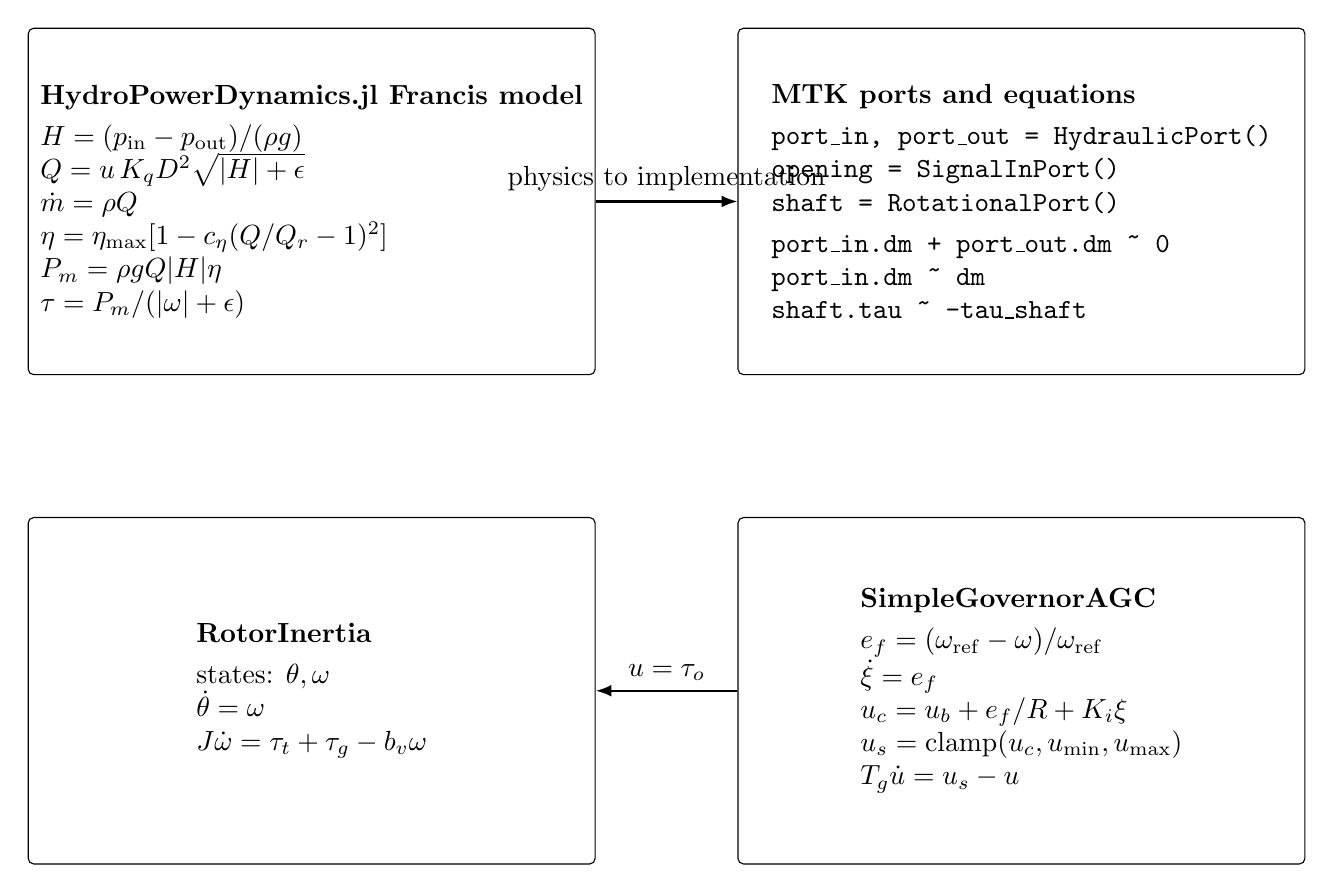
\begin{tikzpicture}[node distance=18mm]

\node[box] (model) {
\textbf{HydroPowerDynamics.jl Francis model}\\[1mm]
$H=(p_{\rm in}-p_{\rm out})/(\rho g)$\\
$Q=u\,K_qD^2\sqrt{|H|+\epsilon}$\\
$\dot m=\rho Q$\\
$\eta=\eta_{\max}[1-c_\eta(Q/Q_r-1)^2]$\\
$P_m=\rho gQ|H|\eta$\\
$\tau=P_m/(|\omega|+\epsilon)$
};

\node[box,right=of model] (code) {
\textbf{MTK ports and equations}\\[1mm]
\texttt{port\_in, port\_out = HydraulicPort()}\\
\texttt{opening = SignalInPort()}\\
\texttt{shaft = RotationalPort()}\\[1mm]
\texttt{port\_in.dm + port\_out.dm \string~ 0}\\
\texttt{port\_in.dm \string~ dm}\\
\texttt{shaft.tau \string~ -tau\_shaft}
};

\draw[arr] (model) -- node[above] {physics to implementation} (code);

\node[box,below=of model] (rotor) {
\textbf{RotorInertia}\\[1mm]
states: $\theta,\omega$\\
$\dot\theta=\omega$\\
$J\dot\omega=\tau_t+\tau_g-b_v\omega$
};

\node[box,right=of rotor] (gov) {
\textbf{SimpleGovernorAGC}\\[1mm]
$e_f=(\omega_{\rm ref}-\omega)/\omega_{\rm ref}$\\
$\dot\xi=e_f$\\
$u_c=u_b+e_f/R+K_i\xi$\\
$u_s=\mathrm{clamp}(u_c,u_{\min},u_{\max})$\\
$T_g\dot u=u_s-u$
};

\draw[arr] (gov.west) -- node[above] {$u=\tau_o$} (rotor.east);
\end{tikzpicture}
\end{document}
